%# -*- coding: utf-8-unix -*-
%%==================================================
%% chapter01.tex for SJTU Master Thesis
%%==================================================

\chapter{绪论}
\label{chap:intro}

\section{论文研究的背景及意义}
\label{sec:intro:analog}
	20 世纪以来,人类生存环境中化学品日益增多,对数量巨大且种类复杂的
	化学物进行健康风险的评估是公共健康领域当前重要的研究课题。此外,人类与
	环境化合物的接触方式多为低剂量下的复合暴露,如何实现高通量的毒性评价和
	科学的风险评估成为研究的热点与难点。
	
		自 2005 年起,美国启动了 21 世纪毒理学研究计划(TOX21),主要借助体
	外测试和计算生物信息学等方法进行高通量化学品毒性评估。然而,使用细胞或
	类器官的体外方法虽然可以进行较高通量的毒性测试,但无法代替动物体内实
	验,因为其结果无法反映化合物进入生物体内吸收、分布、代谢与排泄环节对毒
	性的影响。传统的动物体内毒性研究结果具有很大的参考意义,但是实验周期长、
	成本高,并且涉及动物保护与伦理。如果进行待测化合物低剂量复合暴露毒性研
	究,需要不同化合物的多剂量进行配伍,基于上述动物实验的局限性,难以进行
	高通量的毒性测试。秀丽隐杆线虫作为一种模式生物,对环境变化非常敏感;其
	生命周期和寿命较短,身体尺寸较小易操作,以大肠杆菌为食易培养,身体透明
	易观察,染色体和基因组较小易分析,生物学信号通路保守,因此近年来线虫被
	广泛应用于重金属、PM2.5、农药、纳米颗粒和有机污染物等环境毒理学研究领
	域。国际上目前已进展到第三阶段的 TOX21 计划也在使用包括线虫在内的模式生
	物对前期结果进行验证,并计划对更多环境化合物进行毒性筛选。
	
		传统的线虫培养方法在液体或琼脂板上进行,需要的线虫数量多,待测化合
	物所需量较大,此外难以对单个线虫实现精确刺激、操控和追踪。微流控体系与
	线虫大小尺度相匹配,有望实现线虫芯片内培养、成像和数据分析等。自从 2011
	年美国启动“类器官芯片”计划之后,以微流控芯片为平台的毒理测试技术发展
	迅速,相比器官芯片平台,线虫芯片是在动物个体水平上进行毒理学研究,具有
	不可替代的优势。
	
\section{秀丽隐杆线虫概述}
	\begin{figure}[h]
	  \centering
	  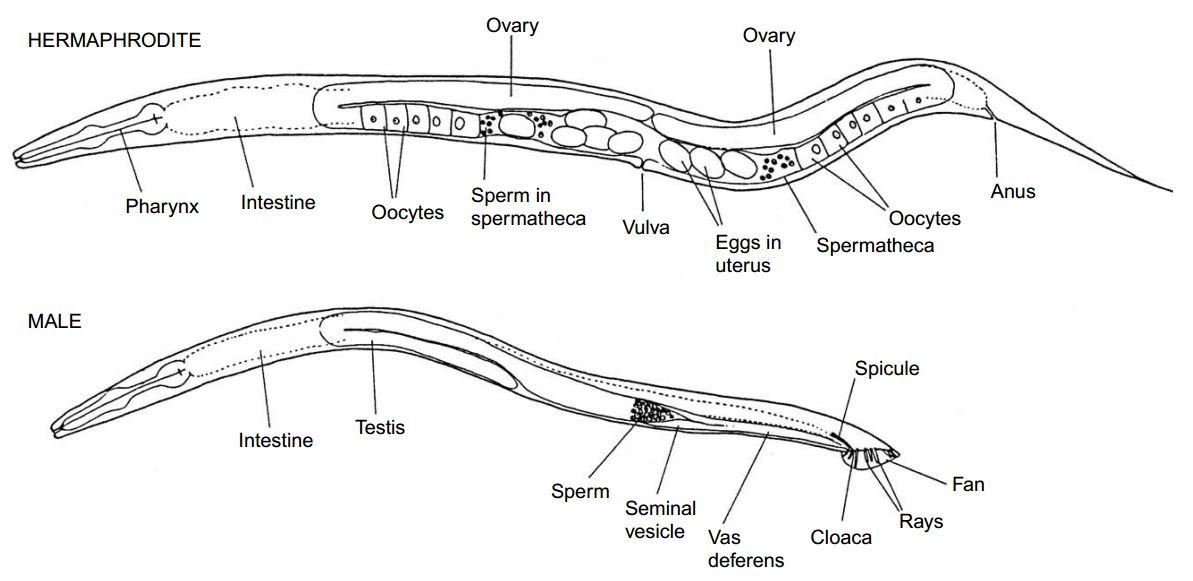
\includegraphics[width=14cm]{figure/chap1/Celegans.jpg}
	  % \hspace{1cm}
	  % 
\includegraphics[width=4cm]{example/sjtulogo.jpg}
	  \bicaption[这里将出现在插图索引中]
		{秀丽隐杆线虫解剖图}
		{Anatomy of adult C.elegans.}
	  \label{fig:Celegans}
	\end{figure}
	秀丽隐杆线虫(简称 C. elegans)是一种微米尺度的无脊椎模式生物,主要生活在土壤中或水中,以大肠杆菌OP50为食,成虫
	体长约为1mm宽度50um,并且从幼虫长到成虫只需要3天。秀丽隐杆线虫是线虫动物门中的一种,包含雌雄同体和雄性两种性别如图\ref{fig:Celegans}。两种性别都是二倍体,都有五对常染色体,
	但雌雄通体的线虫有两个X常染色体(XX)而雄性线虫只有一个X常染色体(XO)。在自然条件下,线虫几乎都为雌雄同体,
	雄性个体只占约五百分之一。线虫的生命周期较为简单如图\ref{fig:lifecycle}所示,成年雌雄同体线虫同时含有精子和卵母细胞,因此能够自体受精。
	每一个自体受精的雌雄同体线虫大约可以产生330多个蛋。如果雄性体线虫交配产蛋量将会提高,并且有利于
	基因的重新组合。在25$^。C$下孵化12个小时即可得到L1期的线虫幼虫,
	长度约为0.15mm。L1期幼虫基本上具备了和成虫一样的器官结构,除了还没有形成生殖器结构,从L1期线虫
	长到L4期只需要3天。
	线虫作为一种现代动物模型被广泛地用于细胞生物学、神经科学、衰老与发育和毒理学等研究中。在2002年
	,研究秀丽线虫的研究团体就已经扩展到300多个实验室,分布在20多个国家和地区。1998年,构成整个基因组的9700万个碱基对DNA的测序基本完成,
	这是第一个经过完整基因组测序的多细胞生物。与其他模式生物相比线虫具有如下技术优势:
	
	\begin{itemize}
	  \item 由于线虫通体透明,可以通过荧光蛋白标记的表达观察细胞的分裂等许多重要的生理过程,
	  还可以用于对神经元成像,研究外部刺激与神经元活动之间的关联。
	  \item 线虫的生命周期短、培养简单以及繁殖能力强,这些特性都有助于加快实验周期,提高实验的并行性。
	  \item 线虫身体构造简单,遗传模式保守,有利于减小实验中由于个体差异而引起实验结果的扰动。
	  \item 对线虫基因的测序已经完成,使得线虫可以在基因筛查分析和其他遗传学实验中发挥重要作用。
	  \item 线虫基因与人类的基因有约40\%的同源性,许多的研究者将线虫作为疾病模型研究疾病机制。
	\end{itemize}
	

	\begin{figure}[h]
	  \centering
	  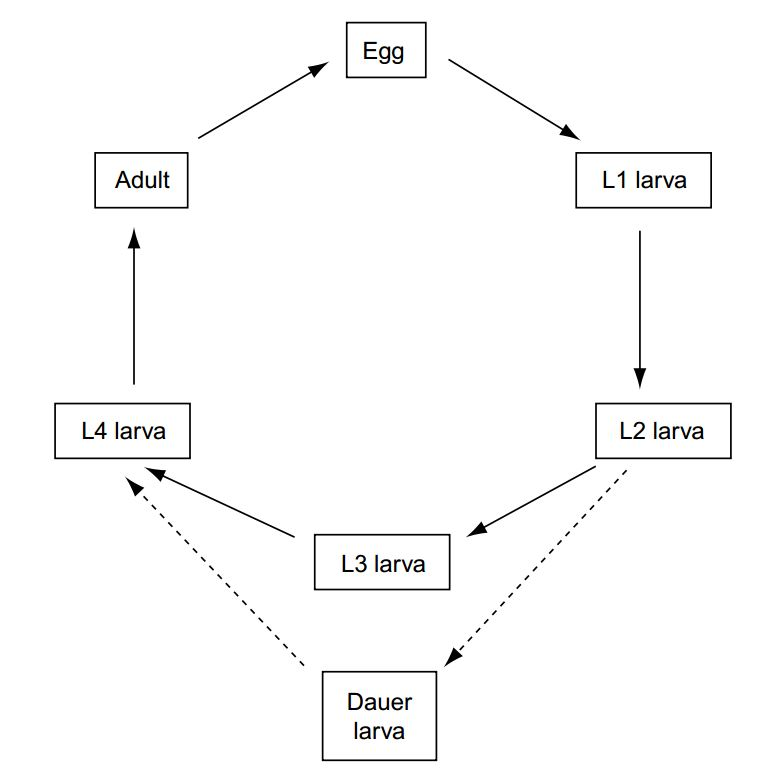
\includegraphics[width=8cm]{figure/chap1/lifecycle.jpg}
	  % \hspace{1cm}
	  % 
\includegraphics[width=4cm]{example/sjtulogo.jpg}
	  \bicaption[这里将出现在插图索引中]
		{秀丽隐杆线虫生命周期}
		{The life cycle of C.elegans.}
	  \label{fig:lifecycle}
	\end{figure}
	
\section{国内外研究现状}
\label{sec:intro:analog}
	微流控是一种在微米尺度操纵流体的技术,具有反应体系小、通量高、自动。化且操作灵活等优势,被越来越多的应用于细胞和微米尺度生物的研究中。
	微流控技术在线虫研究中的应用为研究者们提供了一个全新的研究平台,极大的促进了相关领域的研究进展。利用微流控技术研究线虫具有的
	优势有:\begin{enumerate*}[label=\itshape\alph*)\upshape]
	\item 利用微流控芯片可以实现在细胞尺度上对线虫的操纵。\quad
	\item 利用微流控芯片可以实现对线虫的快速固定与成像,与使用药物麻醉的方法相比,这种固定
		方式不会对线虫产生任何损害,线虫可以在后续步骤中恢复。\quad
	\item 利用微流芯片可以快速的从上千只线虫中的筛选出需要的表型,实现线虫的分选。\quad
	\item 微流控芯片可以为线虫的培养提供精确的微环境,为线虫的感知实验提供精确的刺激传达。\quad
\end{enumerate*}
	结合
	
\subsection{线虫的分选}
\label{sec:intro:analog}
	线虫的筛选往往是基于某种表型,如尺寸、趋电性、趋化性、运动能力、电生理学特性等。
	可从以下角度分类。
	\begin{itemize}
	  \item 有许多文献基于线虫的大小从而对幼虫和成虫进行分选。
	  \item 线虫的趋电性的不同导致线虫向不同的电极靠近从而达到分选的目的,文献若干。
	  \item 基于神经元活动和电生理特性的筛选。
	  \item 区别于物理固定和可逆凝胶固定线虫,研究者提出了一种将液滴捕获用于线虫的分选。
	\end{itemize}
	
\subsection{线虫的固定与成像}
\label{sec:intro:analog}
	按照以下角度综述。
	\begin{itemize}
	  \item 通过PDMS膜形变将线虫限制在一个通道里文献。
	  \item 通过二氧化碳扩散的方式麻醉线虫文献。
	  \item 锥形通道固定线虫文献。
	  \item 最后对幼虫和线虫胚胎的固定文献。
	\end{itemize}

\subsection{线虫行为实验}
\label{sec:intro:analog}
	目前已经有学者研究过的行为包括:线虫的机械感受器、渗透逃避、趋化性、趋电性、觅食反应
热反应、产软行为、繁殖行为等。
	\begin{itemize}
	  \item 线虫的机械感受:如测量线虫肌肉的力度。
	  \item 趋化性,如很多梯度芯片被提出用于相关的研究
	  \item 探讨线虫在拥挤环境下的行为反应
	  \item 趋电性行为,虫子在电场的来回切换下来回运动有助于延长线虫寿命。
	\end{itemize}
\subsection{药物筛选与毒理实验}
\label{sec:intro:analog}
	很多的线虫芯片被开发,用于药物识别,筛选、以及研究毒性对线虫行为、生理电信号衰老。抗菌和代谢
活动身体毒性的影响。
	\begin{itemize}
	  \item 多种复合药物浓度梯度的药物筛选。
	  \item 将线虫暴露在细菌病原体环境中。
	  \item 将线虫暴露在重金属环境中
	\end{itemize}

\section{存在的问题}
\label{sec:intro:analog}
	\begin{itemize}
	  \item 片上梯度的形成
	  \item 游动线虫轮廓的分割
	  \item 一个集成微流控芯片和多线虫实时图像处理的平台还报道的比较少
	\end{itemize}
\section{研究内容}
\label{sec:intro:org}
	\begin{itemize}
	  \item 首先搭建了一个基于微流控芯片的硬件平台
	  \item 设计了一款及线虫轮廓分割、跟踪及特征提取等功能的自动化图像处理软件。
	  并针对线虫分割的鲁棒性与实时性的要求,还提出了一种基于深度学习的线虫轮廓分割的网络。
	  \item 在搭建的硬件平台上,并通过双氧水实验验证 系统的优势。
	\end{itemize}
\section{论文章节安排}
\label{sec:intro:org}
